\section{Engine-based diagnosis of action masking}
\label{sec:jesper-mask-audit}
\contributionauthor{Jesper Eggers}

\subsection{Question and experimental construction}
\contributionauthor{Jesper Eggers}
Both agents restrict the actions available to their Q-networks. This
restriction also enters the Double DQN bootstrap target, so the mask
affects exploration, evaluation, and the value function being learned.
A useful mask must balance two errors: admitting actions that make
survival impossible and excluding actions that permit escape. A restrictive
mask need not achieve the latter balance better. We tested whether the
final agent's temporal search improves this balance relative to RUEHL's
geometric and immediate-danger checks.

We generated 3,000 states, equally divided among crate-placement
probabilities 0, 0.30, and 0.75 on the configured $17\times17$ board.
The focal agent occupies a randomly selected free tile; one to three other
bombs have timers sampled from zero through three. Approximately one
quarter of states also contain a bomb beneath the focal agent. Nearby
bomb placements are oversampled to expose local hazards. All generation
parameters and the fixed seed are retained in the supplementary scripts.

These are stress-test states, not observations sampled from either policy.
They contain no opponents, visible coins, or initially active explosions,
and no new bombs appear after the candidate first action. The test measures
conditional escape feasibility, including a hypothetical own bomb for
\texttt{BOMB}; it does not measure attack quality or how frequently these
hazards arise during competitive play.

\subsection{Reference calculation and metrics}
\contributionauthor{Jesper Eggers}
For each state and first action, the reference asks whether any legal
continuation survives six environment steps. A reachability search
propagates possible positions through terrain, bomb occupancy, and lethal
tiles computed with the engine's actual \texttt{update\_explosions} and
\texttt{update\_bombs} methods. In this engine, blasts pass through
destructible crates and stop at stone walls. Destroyed crates become
traversable on the following action step. Waiting on a bomb beneath the
agent remains legal; moving back onto an occupied bomb tile does not.

A timer-zero bomb explodes after the next action; timer one explodes after
the second action. The blast is lethal on its creation step and the
following action step. A newly placed bomb also decrements during
placement; six steps cover its complete lethal period without further
bombs. Assertions verify timing, terrain, and the distinction between
lethal explosions and harmless smoke. All 265 surviving witness paths
replayed through the engine executed legally and avoided lethal explosions.

Of the generated states, 2,453 admit at least one surviving movement or
waiting continuation. We compute the principal diagnostics on these
recoverable states, so a mask is not penalized where every choice is
already doomed. An admitted action is unsafe when the reference finds
no surviving continuation. The unsafe-admission fraction divides these
errors by all admitted actions in the relevant category. The exclusion
fraction divides viable movement and waiting actions rejected by the mask
by all viable movement and waiting actions. Bombs are assessed separately:
usefulness constraints can correctly exclude a survivable but strategically
pointless placement. Actions from the same state are correlated, so these
fractions describe this benchmark rather than independent Bernoulli trials.

\begin{table}[htbp]
\centering\small
\begin{tabularx}{\textwidth}{@{}Yrr@{}}
\toprule
Diagnostic & RUEHL mask & Final-agent mask \\
\midrule
Unsafe admitted movement/wait & $84/6103$ (1.38\%) & $1/6367$ (0.02\%) \\
Unsafe admitted bombs & $53/712$ (7.44\%) & $0/669$ (0.00\%) \\
Viable movement/wait excluded & $350/6369$ (5.50\%) & $3/6369$ (0.05\%) \\
\bottomrule
\end{tabularx}
\caption{Measured diagnostics on 2,453 recoverable states from the 3,000-state suite. Each fraction uses its own candidate-action denominator.}
\label{tab:jesper-mask-audit}
\end{table}


\subsection{Measured results and failure mechanisms}
\contributionauthor{Jesper Eggers}
RUEHL admits 84 unsafe movement or waiting actions and 53 unsafe bomb
placements; the final mask admits one and zero, respectively
(Table~\ref{tab:jesper-mask-audit}). RUEHL excludes 350 viable movement
or waiting actions, compared with three for the final mask. The final
mask improves both diagnostics here, showing that its longer-horizon
constraints need not retain fewer viable actions.

\begin{figure}[!htbp]
\centering
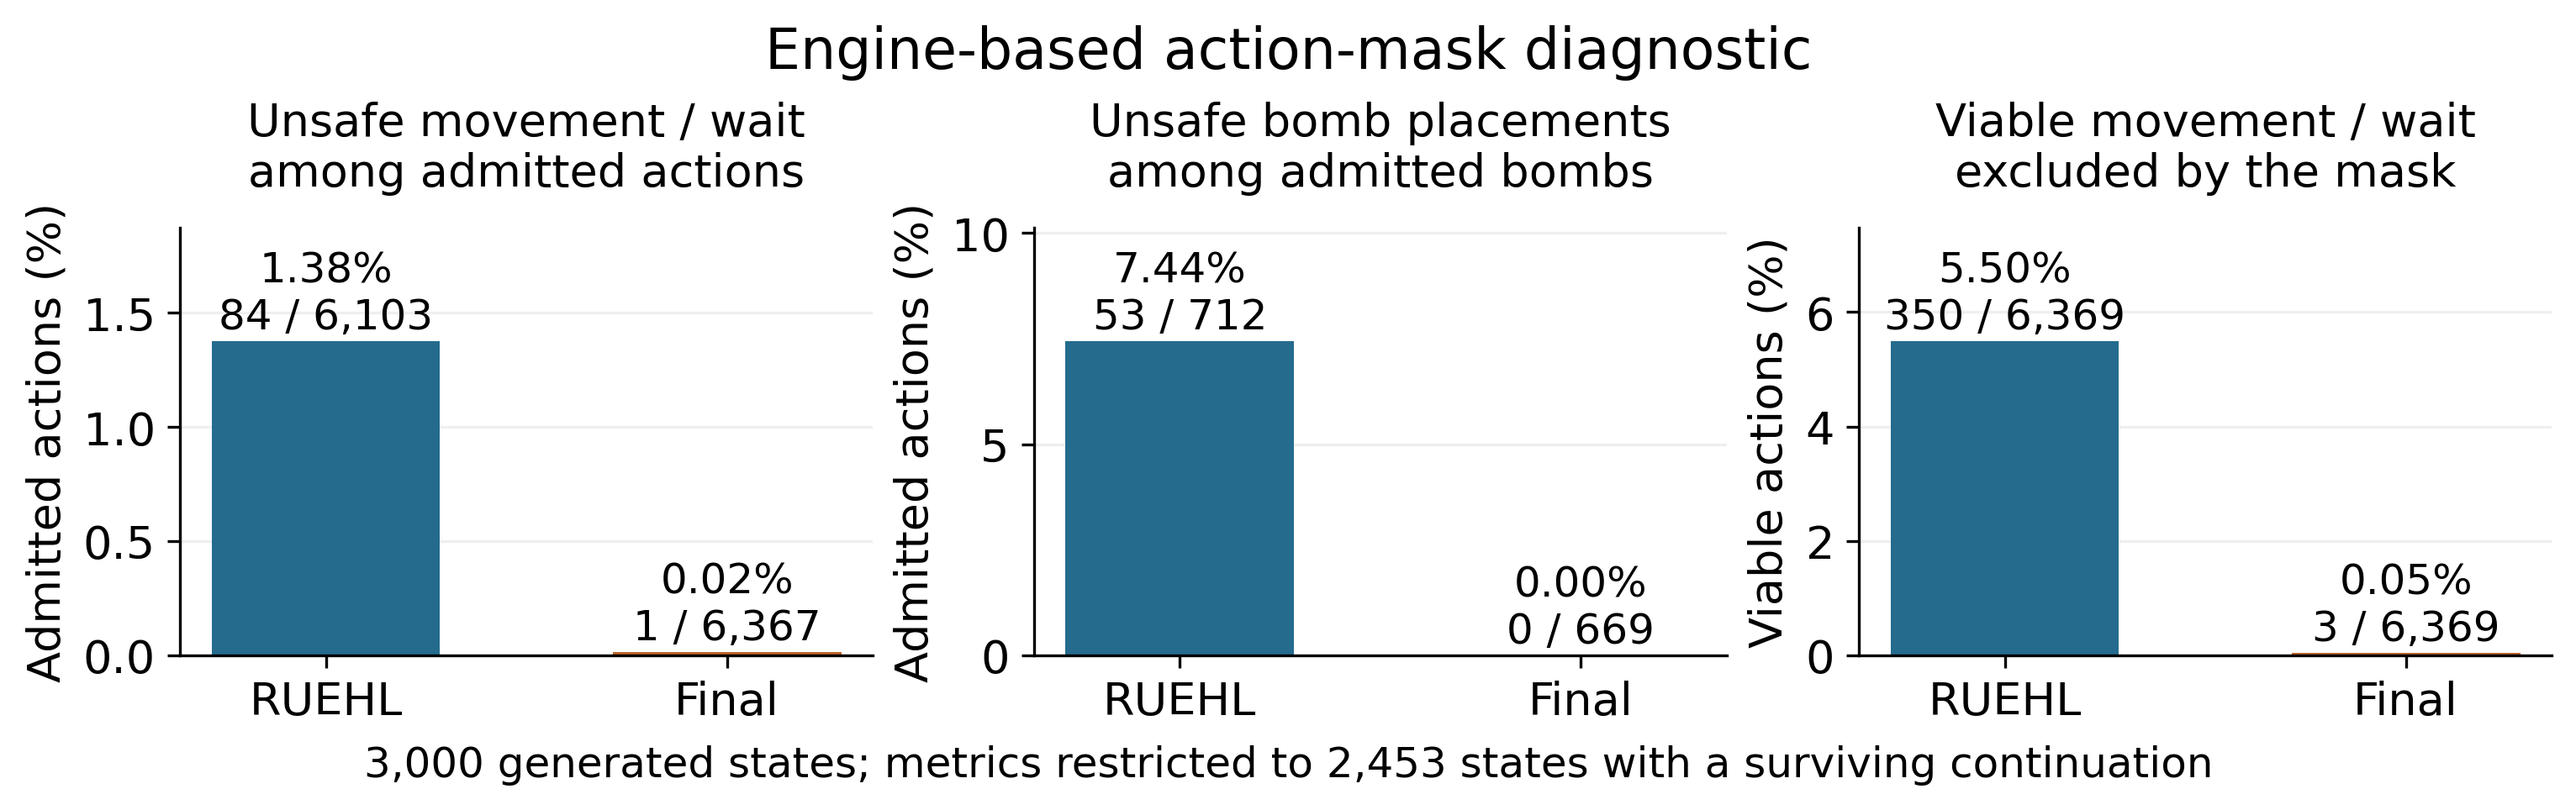
\includegraphics[width=\textwidth]{figures/mask_audit_comparison.png}
\caption{Observed action-level diagnostics from the generated suite. Counts
and denominators are shown explicitly; these are not measured gameplay
death rates.}
\label{fig:jesper-mask-comparison}
\end{figure}

The counterexample in Figure~\ref{fig:jesper-mask-counterexample} explains
how these errors can interact. The agent stands at $(9,8)$, while a bomb
at $(9,6)$ has timer one. Moving down to $(9,9)$ and then right to $(10,9)$
escapes before the existing bomb explodes. RUEHL excludes the initial
downward move because its immediate-danger set already includes the
blast of timer-one bombs. Nevertheless, its separate bomb-placement test
finds a geometric route outside the proposed own blast without jointly
checking the existing bomb's future timing. The resulting mask admits
only \texttt{BOMB}. The reference finds no surviving continuation for
that action, and the final-agent mask instead admits \texttt{DOWN}.
Here, the network cannot correct the mistake: the mask removes the viable
choice before Q-values are compared.

\begin{figure}[!htbp]
\centering
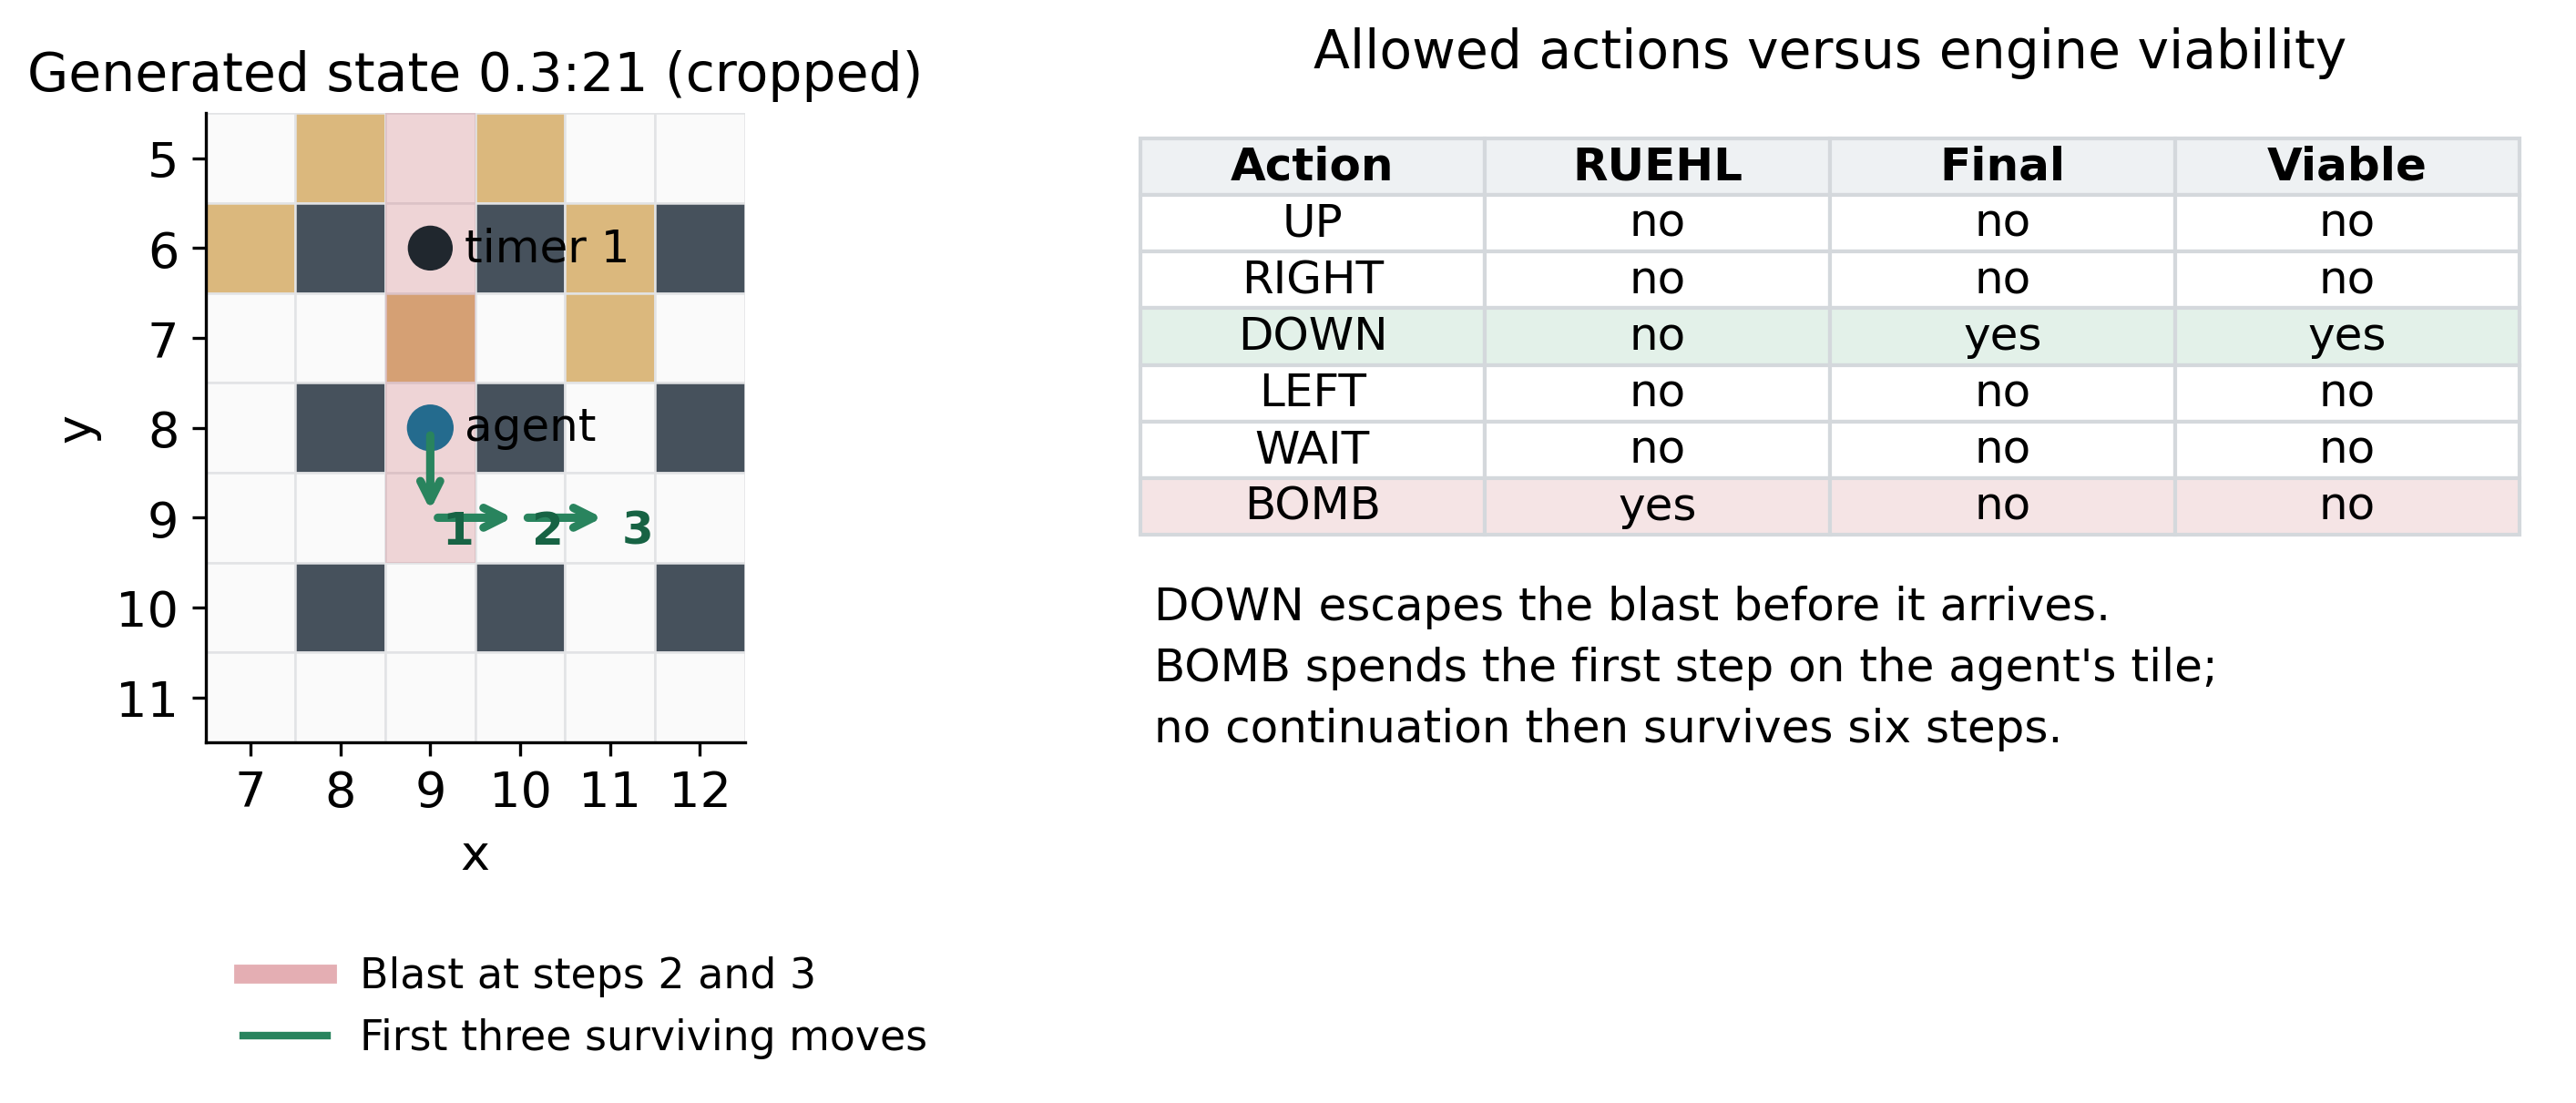
\includegraphics[width=\textwidth]{figures/mask_audit_counterexample.png}
\caption{A recorded generated counterexample, not a tournament replay.
The board is cropped; all bombs on the full board enter the reference
calculation. Green arrows show the first three moves of a surviving
continuation beginning with \texttt{DOWN}.}
\label{fig:jesper-mask-counterexample}
\end{figure}

The final mask's residual unsafe admission occurs in state
\texttt{0.75:428}. Its search keeps crates permanently blocking, missing a
route opened by an existing bomb. All movement and waiting searches fail,
so the fallback restores physically legal movement, including an unsafe
upward move and viable leftward move. Predicting terrain updates would
address this implementation defect.

\subsection{Implications and limits}
\contributionauthor{Jesper Eggers}
The diagnostic establishes that the temporal mask better preserves
six-step escape possibilities under the specified hazard evolution. It
also exposes a repairable implementation defect: static terrain can
trigger a permissive fallback despite a dynamically available escape.

A viable continuation is an existential result. The network may select
different later actions, and opponent movement or new bombs may invalidate
the path. Consequently, generated-state accuracy does not directly predict
competitive survival. The following experiment measures deployment
consequences by holding final-network weights fixed and crossing learned
ranking with the two masks. Claims about learning would additionally
require consistent next-state masking in the Double DQN target and matched
retraining. These diagnostic results establish constraint quality under
the reference dynamics, rather than a ranking of complete trained agents.
\FloatBarrier
